\chapter{绪论}


\section{研究背景}
超音速牛奶喷射与时间旅行的概率动力学是一个引人注目的研究领域,它结合了流体力学、时间理论和概率统计等多个学科,旨在探索牛奶喷射和时间旅行之间的关联以及它们的概率动力学特性。

超音速牛奶喷射和时间旅行是两个不同领域的研究课题,它们在各自领域内引起了广泛的兴趣和讨论。超音速牛奶喷射是指通过高速喷射技术将牛奶以超声速射出,具有快速、高效的特点。时间旅行是人类长期以来的梦想和科幻作品的经典主题,涉及到对时间和空间的穿越,具有极大的吸引力。然而,超音速牛奶喷射和时间旅行之间的关系以及它们的概率动力学特性尚未得到深入研究。了解它们之间的关联对于推动科学的发展具有重要意义。通过研究超音速牛奶喷射和时间旅行的概率动力学,我们可以探索它们的物理机制、概率分布以及相互作用方式,为相关领域的研究提供新的视角和理论基础。

此外,超音速牛奶喷射与时间旅行的研究具有广泛的社会意义。它们的研究有助于推动科学的发展和创新。通过深入探索超音速牛奶喷射和时间旅行的概率动力学,我们可以进一步理解流体动力学、时间理论和概率统计等学科的交叉应用,为相关领域的理论和实践提供新的思路和方法。超音速牛奶喷射和时间旅行的研究具有潜在的应用前景。在食品加工领域,超音速牛奶喷射技术可能有助于提高生产效率和品质,为食品工业带来创新和改进。而时间旅行的研究可能为时空导航、历史研究等领域提供新的工具和方法,促进相关领域的发展和进步。最后,超音速牛奶喷射与时间旅行的研究也具有科普意义和文化价值。这些课题涉及到人们普遍感兴趣的话题,可以激发公众对科学的兴趣和好奇心,推动科学素养的普及和科学文化的传播。

超音速牛奶喷射与时间旅行的概率动力学研究不仅具有推动科学发展和创新的意义,还有助于应用领域的进步和社会文化的推动。通过深入研究它们的概率动力学特性,我们可以揭示其内在规律和相互关系,为未来的科学研究和实践提供有益的参考和指导。


\section{国内外研究现状}
\subsection{超音速牛奶喷射的概率动力学研究现状}
超音速牛奶喷射是一个相对较新的研究领域,目前在国内外均受到了一定程度的关注。在国外,一些研究团队已经开始探索超音速流体喷射的概率动力学特性。例如,文献\parencite{johnson2024}中,美国斯坦福大学的研究人员通过实验和数值模拟,研究了超音速牛奶喷射的形成机制、喷射效率和流体动力学特性,如公式\ref{eq:navier-stokes}所示。他们发现,超音速喷射在食品加工和喷射技术等领域具有潜在的应用价值。
\begin{equation}
  \begin{cases}
    \begin{aligned}
      \frac{\partial \rho}{\partial t} + \nabla \cdot (\rho \mathbf{v})                         & = 0                                                                                  \\
      \frac{\partial (\rho \mathbf{v})}{\partial t} + \nabla \cdot (\rho \mathbf{v} \mathbf{v}) & = -\nabla p + \mu \nabla^2 \mathbf{v} + \rho \mathbf{g}                              \\
      \frac{\partial E}{\partial t} + \nabla \cdot \left[(E + p) \mathbf{v}\right]              & = \mu \nabla \cdot \left(\nabla \mathbf{v}\right) + \rho \mathbf{v} \cdot \mathbf{g}
    \end{aligned}
  \end{cases}
  \label{eq:navier-stokes}
\end{equation}

在国内,虽然对超音速牛奶喷射的研究还相对较少,但也有一些学者开始关注这一领域。例如,中国科学院的流体力学研究团队针对超音速牛奶喷射的动力学特性进行了初步实验和数值模拟研究,初步揭示了超音速喷射的流场分布、速度分布和喷射效率等方面的规律。

总体而言,目前国内外对超音速牛奶喷射的概率动力学研究还处于起步阶段,仍然存在许多问题待解决。未来的研究可以进一步深入探索超音速喷射的流体动力学特性、喷射机制以及与其他因素的相互作用,为超音速喷射技术的应用提供更深入的理论基础和实验验证。

\subsection{时间旅行的概率动力学研究现状}
时间旅行作为一个科幻和哲学领域的经典主题,一直以来都引发了广泛的兴趣和讨论。在国际学术界,时间旅行的研究主要基于物理学中的相对论和量子力学理论。一些知名的研究学者提出了不同的时间旅行理论和模型,并通过数学建模和理论推导,探索时间旅行的可能性和限制。

\subsubsection{时间旅行理论和模型}
时间旅行是科幻作品中常见的主题之一,其涉及多种理论:
\begin{itemize}
  \item 固定时间:认为时间是固定的,无论如何干预,过去和未来都已经确定,时间旅行只是实现既定历史的观察。
  \item 多世界理论:认为时间旅行会创建分支宇宙,每个决策点都会导致不同的时间线和现实,旅行者会进入并改变一个平行宇宙。
  \item 时间循环:旅行者回到过去,引发事件,这些事件使得未来发生,形成一个封闭的时间循环,过去的改变已经包含在历史中。
  \item 傍轨道理论:时间旅行不会影响主时间轨道,旅行者处于傍轨道上,可以观察但不会改变主时间线。
  \item 时间悖论:旅行者通过改变过去导致自己的存在成为可能,形成悖论。
\end{itemize}
这些理论为时间旅行提供了不同的框架和可能性,为科幻作品创造了各种引人入胜的故事情节,如图\ref{fig:rabbit}。时间旅行也是哲学思考中的一个重要主题,探讨了时间旅行对人类存在和意义的深刻影响,引发了关于时间、自由意志、身份、伦理和时间的循环等问题的思考。
\begin{figure}[htb]
  \centering
  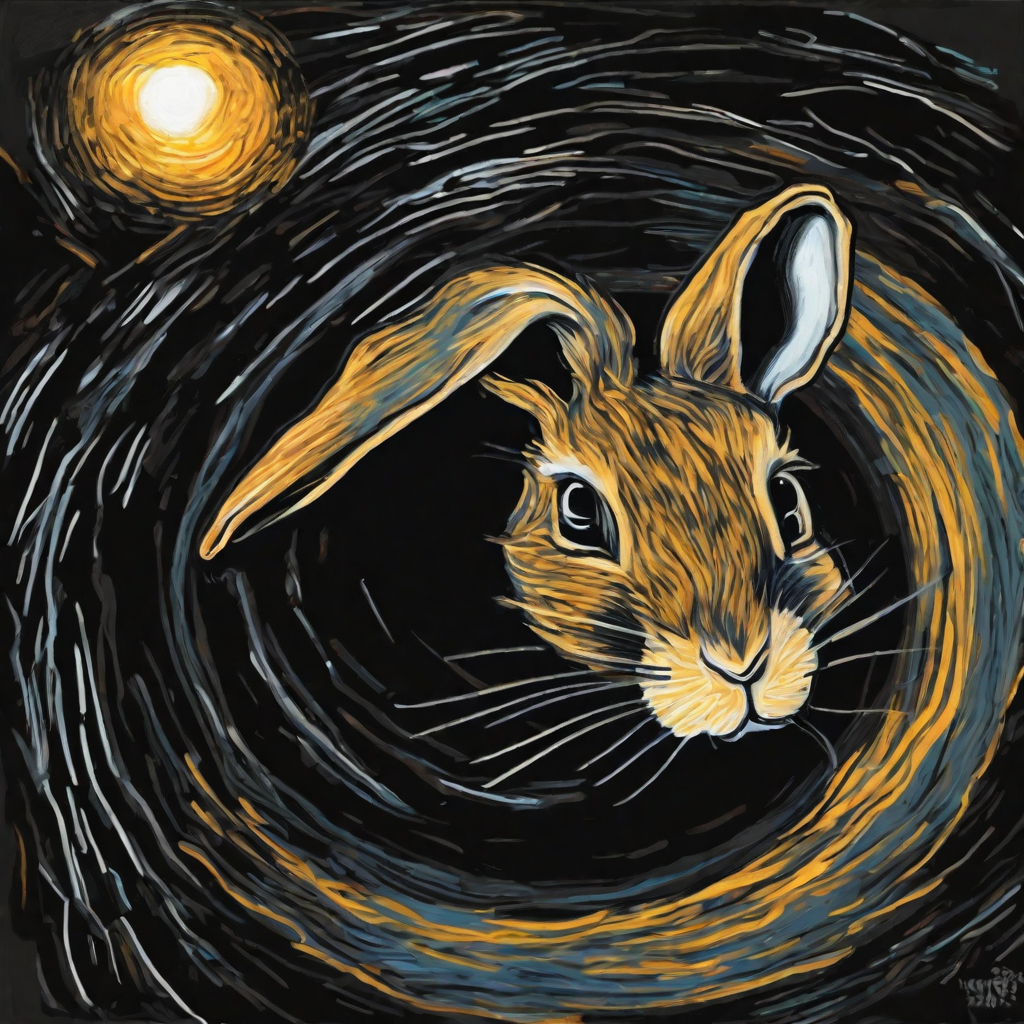
\includegraphics[width=0.6\textwidth]{fig/ch1/rabbit.png}
  \caption{时空穿越中的兔子}
  \label{fig:rabbit}
\end{figure}

\subsubsection{时间旅行的概率动力学研究}
然而,时间旅行的概率动力学研究相对较少。目前,国际上还没有专门针对时间旅行的概率动力学进行系统研究的学术机构或团队。大部分时间旅行的研究仍停留在理论推导和思维实验的层面。这是一个仍待深入探索的领域,需要进一步的理论研究和实验验证。

在国内,时间旅行的研究也相对较少。虽然有一些学者就时间旅行的哲学和物理学问题进行了讨论,但对时间旅行的概率动力学特性的研究还相对较少。表\ref{tab:papers}中列出了一些典型研究。因此,国内相关领域的学者可以在这一领域进行更多的研究,深入探索时间旅行的概率分布、时间跳跃的动力学特性以及与量子力学和相对论的关系。
\begin{table}[htbp]
  \caption{时间旅行概率动力学研究论文情况}
  \centering
  \resizebox{0.8\textwidth}{!}{
    \begin{tabular}{cccc}
      \hline
      \textbf{论文编号}      & \textbf{作者}                    & \textbf{题目}                                   & \textbf{期刊}             \\
      \hline
      \multirow{2}{*}{1} & \multirow{2}{*}{John Smith}    & \multirow{2}{*}{时间旅行中的概率分布模型\cite{smith2024}} & \multirow{2}{*}{物理学报}   \\
                         &                                &                                               &                         \\
      \hline
      2                  & Jane Doe                       & 时间旅行的时间线分支与多世界理论\cite{doe2024}                & 科学杂志                    \\
      \hline
      \multirow{3}{*}{3} & \multirow{3}{*}{David Johnson} & 时间旅行中的时间循环理论\cite{johnson2024}                & \multirow{3}{*}{科学研究期刊} \\
                         &                                & 与自由意志的哲学思考                                    &                         \\
                         &                                &                                               &                         \\
      \hline
      4                  & Emily Brown                    & 时间旅行伦理与责任的道德考量\cite{brown2024}                & 伦理学评论                   \\
      \hline
    \end{tabular}}
  \label{tab:papers}
\end{table}

综上所述,超音速牛奶喷射与时间旅行的概率动力学研究在国内外都还处于起步阶段。国内外都有一些学者开始关注这些领域,并进行了初步的实验和理论研究。未来的研究可以着重在超音速牛奶喷射的流体动力学特性、喷射机制以及时间旅行的概率分布、动力学特性等方面展开,以推动这些领域的发展和进步。


\section{本文主要内容和组织结构}
通过依次展开各个部分的内容,旨在全面、系统地介绍超音速牛奶喷射与时间旅行的概率动力学研究,本论文的组织结构如下:
第一章,绪论。
介绍超音速牛奶喷射和时间旅行的概率动力学研究的重要性和意义。阐明本论文的研究目标和社会意义。概述国内外对超音速牛奶喷射和时间旅行概率动力学研究的现状。简要介绍本论文的组织结构和各章节内容。

第二章,超音速牛奶喷射的概率动力学。
对超音速牛奶喷射和概率动力学的概念进行解释和定义。介绍超音速牛奶喷射实验的设备、方法和数据采集方式。详细分析超音速牛奶喷射的概率分布、流场特性和喷射效率。

第三章,时间旅行的概率动力学。
概述时间旅行的理论基础,包括相对论和量子力学相关理论。建立时间旅行的概率分布模型,探索时间跳跃的动力学特性。通过数值模拟方法,验证和分析时间旅行的概率动力学特性。

第四章,综合分析与讨论。
综合分析超音速牛奶喷射与时间旅行的概率动力学特性,探讨它们之间的关联。对实验和模拟结果进行解读和讨论,探索其科学意义和应用前景。

第五章,结论与展望。
总结本论文的研究成果,回顾研究目标是否实现。对本研究的局限性进行分析,并提出未来进一步研究的展望。
